\documentclass[preview]{standalone}
\usepackage{ctex}

%graphics
\usepackage{xcolor}
\usepackage{tikz}
\usetikzlibrary{shapes.geometric, shapes.multipart, arrows, calc, through}
\usetikzlibrary{3d}
\usepackage[caption=false,font=footnotesize]{subfig}

\colorlet{dot-color}{black!80}
\tikzset{
    pics/cell/.style = {
        code = {%
        \coordinate (-center) at (0,0);
        
        \fill +(-0.45,-0.45) coordinate(-sw) 
           -- +(-0.45, 0.45) coordinate(-nw)
           -- +( 0.45, 0.45) coordinate(-ne)
           -- +( 0.45,-0.45) coordinate(-se)
           -- cycle;
        \coordinate (-swo) at ($ (-center)!0.5!(-sw) $);
        \coordinate (-nwo) at ($ (-center)!0.5!(-nw) $);
        \coordinate (-neo) at ($ (-center)!0.5!(-ne) $);
        \coordinate (-seo) at ($ (-center)!0.5!(-se) $);
        
        \coordinate (-south) at ($ (-sw)!.5!(-se) $);
        \coordinate (-north) at ($ (-nw)!.5!(-ne) $);
        \coordinate (-west)  at ($ (-sw)!.5!(-nw) $);
        \coordinate (-east)  at ($ (-se)!.5!(-ne) $);
        
        \fill[white] (-swo) let \p1=($ (-center)!.5!(-swo) $) in circle ({veclen(\x1,\y1)});
        \fill[white] (-nwo) let \p1=($ (-center)!.5!(-nwo) $) in circle ({veclen(\x1,\y1)});
        \fill[white] (-neo) let \p1=($ (-center)!.5!(-neo) $) in circle ({veclen(\x1,\y1)});
        \fill[white] (-seo) let \p1=($ (-center)!.5!(-seo) $) in circle ({veclen(\x1,\y1)});
        
        \ifnum#1=1\relax
            \fill[dot-color] (-swo) let \p1=($ (-center)!.32!(-swo) $) in circle ({veclen(\x1,\y1)});
            \fill[dot-color] (-neo) let \p1=($ (-center)!.32!(-neo) $) in circle ({veclen(\x1,\y1)});
        \else
            \ifnum#1=-1\relax
                \fill[dot-color] (-nwo) let \p1=($ (-center)!.32!(-nwo) $) in circle ({veclen(\x1,\y1)});
                \fill[dot-color] (-seo) let \p1=($ (-center)!.32!(-seo) $) in circle ({veclen(\x1,\y1)});
            \else
                \fill[dot-color] (-swo) let \p1=($ (-center)!.22!(-swo) $) in circle ({veclen(\x1,\y1)});
                \fill[dot-color] (-nwo) let \p1=($ (-center)!.22!(-nwo) $) in circle ({veclen(\x1,\y1)});
                \fill[dot-color] (-neo) let \p1=($ (-center)!.22!(-neo) $) in circle ({veclen(\x1,\y1)});
                \fill[dot-color] (-seo) let \p1=($ (-center)!.22!(-seo) $) in circle ({veclen(\x1,\y1)});
            \fi
        \fi
        }
    },
    pics/cell/.default={0},
    pics/cross_cell/.style = {
        code = {%
        \coordinate (-center) at (0,0);
        \fill +(-0.45,-0.45) coordinate(-sw) 
           -- +(-0.45, 0.45) coordinate(-nw)
           -- +( 0.45, 0.45) coordinate(-ne)
           -- +( 0.45,-0.45) coordinate(-se)
           -- cycle;
        \coordinate (-n) at ($(-ne)!0.5!(-nw)$);
        \coordinate (-s) at ($(-se)!0.5!(-sw)$);
        \coordinate (-e) at ($(-ne)!0.5!(-se)$);
        \coordinate (-w) at ($(-nw)!0.5!(-sw)$);
        
        \coordinate (-no) at ($(-center)!0.65!(-n)$);
        \coordinate (-so) at ($(-center)!0.65!(-s)$);
        \coordinate (-eo) at ($(-center)!0.65!(-e)$);
        \coordinate (-wo) at ($(-center)!0.65!(-w)$);

        \fill[white] (-no) let \p1=($ (-center)!0.5!(-no) $) in circle ({veclen(\x1,\y1)});
        \fill[white] (-so) let \p1=($ (-center)!0.5!(-so) $) in circle ({veclen(\x1,\y1)});
        \fill[white] (-eo) let \p1=($ (-center)!0.5!(-eo) $) in circle ({veclen(\x1,\y1)});
        \fill[white] (-wo) let \p1=($ (-center)!0.5!(-wo) $) in circle ({veclen(\x1,\y1)});
        
        \ifnum#1=1\relax
                \fill[dot-color] (-no) let \p1=($ (-center)!.32!(-no) $) in circle ({veclen(\x1,\y1)});
                \fill[dot-color] (-so) let \p1=($ (-center)!.32!(-so) $) in circle ({veclen(\x1,\y1)});
        \else
            \ifnum#1=-1\relax
                \fill[dot-color] (-eo) let \p1=($ (-center)!.32!(-eo) $) in circle ({veclen(\x1,\y1)});
                \fill[dot-color] (-wo) let \p1=($ (-center)!.32!(-wo) $) in circle ({veclen(\x1,\y1)});
            \fi
        \fi
        }
    },
}

%from Torres
\definecolor{clock0}{HTML}{008000}
\definecolor{clock1}{HTML}{800080}
\definecolor{clock2}{HTML}{008080}
\definecolor{clock3}{HTML}{F2F2F2}
\definecolor{input}{HTML}{3663B2}
\definecolor{output}{HTML}{D47000}
\definecolor{fixed}{HTML}{000000}


\begin{document}

\begin{figure}[!t]
\centering
\subfloat[共面交叉]{
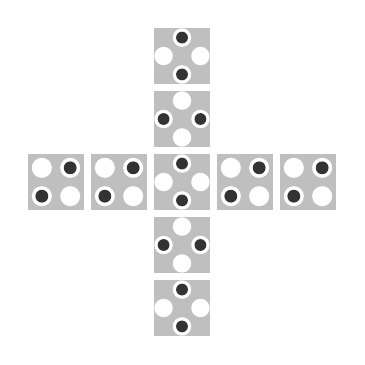
\begin{tikzpicture}[scale=0.8,transform shape]
    \pic[gray!50] at (0,0){cell=1};
    \pic[gray!50] at (1,0){cell=1};
    \pic[gray!50] at (3,0){cell=1};
    \pic[gray!50] at (4,0){cell=1};
    
    \pic[gray!50] at (2,0){cross_cell=1};
    \pic[gray!50] at (2,1){cross_cell=-1};
    \pic[gray!50] at (2,-1){cross_cell=-1};
    \pic[gray!50] at (2,2){cross_cell=1};
    \pic[gray!50] at (2,-2){cross_cell=1};
 
\end{tikzpicture}
}
\hfil
\subfloat[多层异面交叉]{
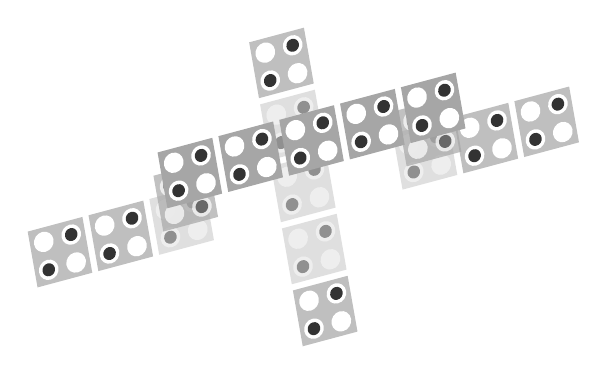
\begin{tikzpicture}[z={(80:3mm)},x={(15:8mm)},y={(100:8mm)}]

\begin{scope}[canvas is xy plane at z=0,transform shape]
    \pic[gray!50] at (0,0) {cell=1};
    \pic[gray!50] at (1,0) {cell=1};
    \pic[gray!50,fill opacity=0.5] at (2,0) {cell=1};
    
    \pic[gray!50] at (4,2) {cell=1};
    \pic[gray!50,fill opacity=0.5] at (4,1) {cell=1};
    \pic[gray!50,fill opacity=0.5] at (4,0) {cell=1};
    \pic[gray!50,fill opacity=0.5] at (4,-1) {cell=1};
    \pic[gray!50] at (4,-2) {cell=1};
    
    \pic[gray!50,fill opacity=0.5] at (6,0) {cell=1};
    \pic[gray!50] at (7,0) {cell=1};
    \pic[gray!50] at (8,0) {cell=1};
\end{scope}

\begin{scope}[canvas is xy plane at z=1, transform shape]
    \pic[gray!70,fill opacity=0.7] at (2,0) {cell=-1};
    \pic[gray!70,fill opacity=0.7] at (6,0) {cell=-1};
\end{scope}

\begin{scope}[canvas is xy plane at z=2, transform shape]
    \pic[gray!70] at (2,0) {cell=1};
    \pic[gray!70] at (3,0) {cell=1};
    \pic[gray!70] at (4,0) {cell=1};
    \pic[gray!70] at (5,0) {cell=1};
    \pic[gray!70] at (6,0) {cell=1};
\end{scope}

\end{tikzpicture}
}

\end{figure}
\end{document}
